\documentclass[10pt]{article}
\usepackage{icmlko}

\icmlmeta{IP 파운데이션 월드모델}{291}{만나지 않는다}{로드맵이 상태 층의 선결과제로 지목한 IP 그래프 --- 열한 도메인이 이름으로 서로 안 만나고, 만나는 자리는 팝업 하나다}

\begin{document}

\twocolumn[
\icmlheader

\begin{abstract}
로드맵이 상태 층(블록 3)의 선결과제로 \textbf{크로스 도메인 IP 그래프}를
지목했다. 그게 실제로 가능한지 열한 도메인의 엔티티 필드를 전부 훑었다
(병렬 조사 넷). \textbf{결론 하나 --- 콘텐츠 도메인끼리는 안 만난다.}
이름 완전일치로 이어지는 작품이 애니↔세계애니 53 · 게임↔모바일 34 ·
\textbf{웹툰↔애니 10}(2,817$\times$2,073 중에서다) · 만화↔게임 \textbf{1} ·
아이돌↔펀딩 \textbf{0} · 책↔펀딩 \textbf{0} 이다. 원인은 명확하다 ---
\textbf{도메인마다 표기가 다르고}(웹툰 한글 · 만화 romaji · 모바일 현지화명)
\textbf{원작·프랜차이즈 필드를 가진 도메인이 하나도 없다.}
\textbf{결론 둘 --- 이미 있는 IP 그래프도 lab 에서는 못 쓴다.}
\texttt{data/state/ip\_graph.json} 에 IP 969개가 있는데 관측이 전부 팝업 ·
시장 · 아이돌 것이고, lab 의 거름망을 통과해 \textbf{두 도메인 이상에 걸치는
IP 는 6개}, \textbf{다른 도메인의 더 이른 라벨을 가진 유보 행은 2개}다.
\textbf{셋 --- 그런데 팝업이 허브다.} 내부 \texttt{brand\_key} 263개에
원피스 · 짱구 · 귀멸의칼날 · 주술회전 · 마비노기 · 메이플스토리 · NCT 가,
시장 \texttt{ip\_or\_collab} 434개에 슈퍼마리오 · 해리포터 · 치이카와가 있다.
조인 코드도 이미 돈다(\texttt{derive\_features.py}, 완전일치). 넓혀 봤다 ---
\textbf{정규화 후 접두사} 규칙으로 서로 다른 IP 23 $\to$ \textbf{40}, 내부
48 $\to$ \textbf{70}, 시장 60 $\to$ \textbf{97} 이고 오탐(``이마트'' 가 긴
설명문에 우연히 든 것)은 접두사 조건이 걷어낸다. 그 조인으로
\texttt{prior\_count} 가 555건 중 \textbf{106건(19\%)} 바뀐다. \textbf{채택
근거(학습 구간 상관)는 $+$0.1392 $\to$ $+$0.2114 로 오르는데} 유보는
$+$0.2042 $\to$ $+$0.2029 로 그대로고 판은 $+$0.0011 · 진짜 0개다.
\textbf{오늘 하루 종일 만난 그 모양이다 --- 고쳤는데 잴 수가 없다.}
\end{abstract}
]

\section{상태 층의 선결과제를 실제로 봤다}

이 실험실의 로드맵에서 남은 벽은 블록 3(상태 층)이고, 프롬프트 주입식
시도가 세 번 기각된 뒤 남은 진단이 ``학습된 가중치라야 한다''였다. 그리고
그 선결과제로 적힌 것이 \textbf{크로스 도메인 IP 그래프}다 --- 같은 IP 가
웹툰에도 팝업에도 나오면 한쪽의 이력이 다른 쪽 예측에 쓰일 수 있다.

\textbf{가능한지부터 봤다.} 열한 도메인의 엔티티 필드를 병렬로 훑었다.

\section{콘텐츠 도메인은 서로 안 만난다}

\begin{figure*}[t]
\centering
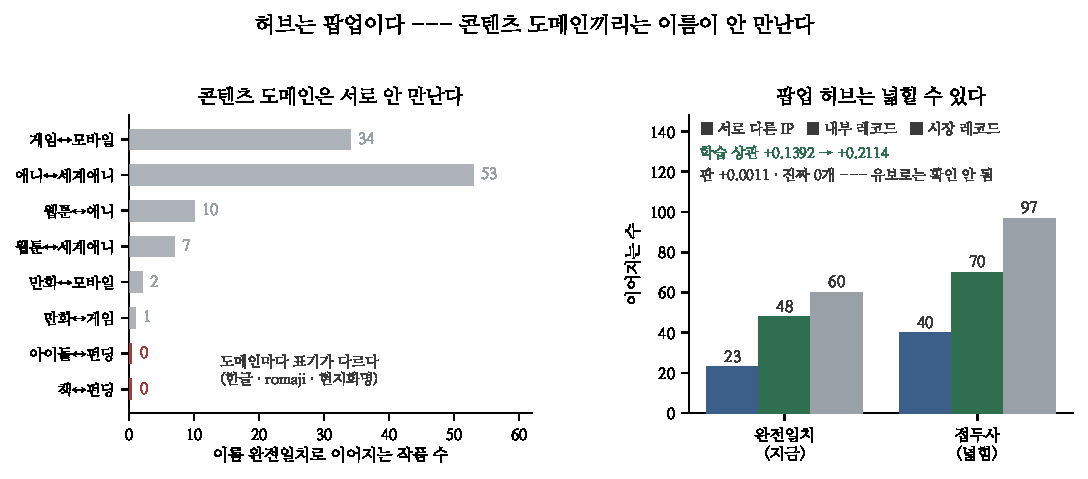
\includegraphics[width=\textwidth]{figs/meet.pdf}
\caption{왼쪽 --- 도메인 쌍마다 이름 완전일치로 이어지는 작품 수. 오른쪽 ---
팝업 두 층의 IP 조인을 넓혔을 때.}
\end{figure*}

\begin{center}\small
\begin{tabular}{lr}
\hline
도메인 쌍 & 이어지는 작품 \\
\hline
애니 $\leftrightarrow$ 세계애니 & 53 \\
게임 $\leftrightarrow$ 모바일 & 34 (회사로는 59) \\
웹툰 $\leftrightarrow$ 애니 & \textbf{10} \\
웹툰 $\leftrightarrow$ 세계애니 & 7 \\
만화 $\leftrightarrow$ 모바일 & 2 \\
만화 $\leftrightarrow$ 게임 & \textbf{1} \\
아이돌 $\leftrightarrow$ 펀딩 & \textbf{0} \\
책 $\leftrightarrow$ 펀딩 & \textbf{0} \\
\hline
\end{tabular}
\end{center}

웹툰 2,817건과 애니 2,073건에서 \textbf{열 개}가 만난다. 원인은 둘이다.

\textbf{① 표기가 다르다.} 웹툰은 한글 제목만, 만화는 romaji 만
(\texttt{Kimetsu no Yaiba}), 모바일은 한국 스토어 현지화명(\texttt{귀멸의
칼날}), 세계애니만 romaji $+$ 원어 $+$ 영문 $+$ 별칭을 다 갖는다. 같은
작품이 세 도메인에서 세 표면형이다.

\textbf{② 원작 · 프랜차이즈 필드를 가진 도메인이 하나도 없다.} 애니의
\texttt{series\_id} 는 도메인 안에서만 쓰는 그룹 키이고, 세계애니의
\texttt{source} 는 원작 \emph{매체 종류}(MANGA · LIGHT\_NOVEL)일 뿐 원작
\emph{제목}이 아니다. 만화의 \texttt{authors} 는 이름이 아니라 AniList
staff 정수 ID 다.

\paragraph{그러니 이건 수집 설계의 결과다} 도메인마다 다른 플랫폼에서
독립으로 긁었고 서로 잇는 키를 안 남겼다. 버그가 아니라 \textbf{그때
필요 없던 것}이다.

\section{이미 있는 IP 그래프도 lab 에서는 못 쓴다}

\texttt{data/state/ip\_graph.json} 이 이미 있다 --- IP 969개, 관측
\texttt{popup\_market} 646 · \texttt{popup\_internal} 380 ·
\texttt{idol\_debut} 271. \textbf{lab 의 세 도메인과 id 가 붙는다}(팝업
68/75 · 시장팝업 205/205 · 아이돌 76/81).

그런데 쓸 수 있는 표본이 없다.

\begin{center}\small
\begin{tabular}{lr}
\hline
ip\_graph 의 교차 도메인 IP & 35 \\
lab 거름망 통과 후 & \textbf{6} \\
\hline
\textbf{다른 도메인의 더 이른 라벨을 가진 유보 행} & \textbf{2} \\
\hline
\end{tabular}
\end{center}

여섯은 킥플립 · 바이탈뷰티 · NCT WISH · 뉴진스 · QWER · 르세라핌이고,
쓸 수 있는 유보 행 둘은 \textbf{둘 다 NCT WISH} 다(시장팝업 2026 $\leftarrow$
아이돌 2024). \textbf{$n{=}2$ 로는 아무것도 못 잰다.}

\section{그런데 팝업이 허브다}

콘텐츠 도메인끼리는 안 만나는데, \textbf{팝업 층에는 그 IP 들이 다 있다.}

\begin{center}\small
\begin{tabular}{ll}
\hline
내부 \texttt{brand\_key} & 263개 · 덮음 100\% \\
& 원피스 · 짱구 · 귀멸의칼날 · 주술회전 \\
& 마비노기 · 메이플스토리 · 쿠키런 · NCT \\
\hline
시장 \texttt{ip\_or\_collab} & 434개 · 덮음 83\% \\
& 슈퍼마리오 · 해리포터 · 치이카와 · 명조 \\
\hline
\end{tabular}
\end{center}

\textbf{팝업은 IP 협업이라 정의상 다른 도메인의 IP 를 데려온다.} 그리고 두
층을 잇는 조인 코드가 \emph{이미 돌고 있다}(\texttt{ingest/derive\_features.py}
의 \texttt{\_ipkey\_int} · \texttt{\_ipkey\_mkt}) --- 그 결과가
\texttt{ip\_history.prior\_count} 이고, 노트 284가 시장팝업의
\texttt{venue\_prominence} 로 태운 바로 그 필드다.

\paragraph{완전일치라 12\% 만 이어진다} 넓혀 봤다.

\begin{center}\small
\begin{tabular}{lrrr}
\hline
규칙 & 다른 IP & 내부 & 시장 \\
\hline
완전일치(지금) & 23 & 48/380 & 60/647 \\
정규화 & 23 & 48 & 60 \\
\textbf{정규화 $+$ 접두사} & \textbf{40} & \textbf{70} & \textbf{97} \\
정규화 $+$ 포함 & 46 & 78 & 105 \\
\hline
\end{tabular}
\end{center}

\textbf{포함까지 가면 오탐이 섞인다} --- ``이마트''가 \emph{도드람한돈브랜드
유튜버정육왕콘텐츠협업\textbf{이마트}푸드마켓고덕점연계}에 우연히 들어 있고,
``하리보''가 브랜드 열거 문장에 들어 있다. \textbf{접두사로 좁히면 그런 것이
사라지고} 좋은 것은 남는다 --- 포켓몬$\to$포켓몬고, 주술회전$\to$주술회전2기,
귀멸의칼날$\to$귀멸의칼날무한성편, 마비노기$\to$마비노기모바일.

\section{고쳤는데 잴 수가 없다}

넓힌 조인으로 \texttt{prior\_count} 가 시장 레코드 555건 중 \textbf{106건
(19\%)} 바뀐다(0 초과 레코드 134 $\to$ 182, 평균 0.69 $\to$ 1.15). 지금
방식은 파일 값을 \textbf{555/555 재현}하므로 구현은 맞다.

\begin{center}\small
\begin{tabular}{lrr}
\hline
& 지금 & 넓힘 \\
\hline
\textbf{학습 구간 상관}(채택 근거) & $+$0.1392 & \textbf{$+$0.2114} \\
유보 상관 & $+$0.2042 & $+$0.2029 \\
\hline
판 & 0.4733 & 0.4745 ($+$0.0011) \\
시장팝업 & 0.2137 & 0.2250 ($t{=}0.36$) \\
진짜 & \multicolumn{2}{c}{\textbf{0개} (t 문턱 2.81)} \\
\hline
\end{tabular}
\end{center}

노트 239 · 285의 규약대로 \textbf{채택 근거는 학습 구간}이고 거기서는
$+$0.14 $\to$ $+$0.21 로 오른다. 그런데 $n{=}101$ 이면 스피어만의 SE 가
0.1 언저리라 그 차이도 문턱 아래이고, 유보는 아예 안 움직인다.

\textbf{오늘 하루 종일 만난 그 모양이다} --- 노트 285의 범주 축($+$0.0167),
노트 282의 아이돌($+$0.0651), 노트 287의 넓힌 팝업($+$0.0076), 그리고 이것.
\textbf{고친 것이 옳다는 증거는 라벨 밖에 있고}(오탐 제거 · 조인율 $+$46\%),
\textbf{그 옳음이 점수로는 안 나온다.}

\paragraph{그래서 안 적용한다 --- 아직} 조인 규칙을 고치면
\texttt{data/records} 와 \texttt{data/market\_records} 의 파생 필드가 다시
쓰이고, 그건 \textbf{lab 과 하네스 두 트랙의 자료를 동시에 바꾼다.} 하네스는
지금 KIOF 전향 사이클이 실측을 기다리는 중이다. \textbf{규칙은 코드로
남기고 적용은 그 사이클 뒤로 미룬다.}

\paragraph{남은 것}
\begin{center}\small
\begin{tabular}{ll}
\hline
갈래 & 왜 \\
\hline
하네스에서 재기 & MAPE 16$\sim$18\% 쪽은 분해능이 다르다 \\
별칭 사전 & 세계애니 synonyms · anime\_match 87건 \\
회사 축 & 게임↔모바일은 회사로 59개 붙는다 \\
KIOF 뒤 적용 & 전향 사이클이 끝나면 \\
\hline
\end{tabular}
\end{center}

\paragraph{규약} \textbf{``상태를 붙이자''는 제안이 나오면 엔티티가 실제로
만나는지 먼저 센다.} 이 실험실은 상태 층을 세 번 시도해 세 번 기각했는데,
\textbf{그 시도들이 전제한 IP 그래프가 lab 에서는 유보 행 두 개짜리였다.}
방법이 아니라 기질(基質)이 없었던 것이다. 그리고 \textbf{허브가 있는 자리를
먼저 본다} --- 콘텐츠 도메인끼리는 0$\sim$53 인데 팝업 층은 263$\times$434 다.

\end{document}
